\documentclass[a4paper, 11pt]{report}
\usepackage{blindtext}
\usepackage[T1]{fontenc}
\usepackage[utf8]{inputenc}
\usepackage{titlesec}
\usepackage{fancyhdr}
\usepackage{geometry}
\usepackage{fix-cm}
\usepackage[hidelinks]{hyperref}
\usepackage{graphicx}
\usepackage{titlesec}
\usepackage{hyperref}
\usepackage{url}
\usepackage[utf8]{inputenc}
\usepackage{amsmath}
\usepackage{amsfonts}
\usepackage{amssymb}
\usepackage{graphicx}
\usepackage{listings}

\usepackage[english]{babel}

\geometry{ margin=30mm }
\counterwithin{subsection}{section}
\renewcommand\thesection{\arabic{section}.}
\renewcommand\thesubsection{\thesection\arabic{subsection}.}
\usepackage{tocloft}
\renewcommand{\cftchapleader}{\cftdotfill{\cftdotsep}}
\renewcommand{\cftsecleader}{\cftdotfill{\cftdotsep}}
\setlength{\cftsecindent}{2.2em}
\setlength{\cftsubsecindent}{4.2em}
\setlength{\cftsecnumwidth}{2em}
\setlength{\cftsubsecnumwidth}{2.5em}

\titlespacing\section{0pt}{12pt plus 4pt minus 2pt}{0pt plus 2pt minus 2pt}
\titlespacing\subsection{0pt}{12pt plus 4pt minus 2pt}{0pt plus 2pt minus 2pt}
\begin{document}
\titleformat{\section}
{\normalfont\fontsize{15}{0}\bfseries}{\thesection}{1em}{}
\titlespacing{\section}{0cm}{0.5cm}{0.15cm}
\titleformat{\subsection}
{\normalfont\fontsize{13}{0}\bfseries}{\thesubsection}{0.5em}{}
\titlespacing{\section}{0cm}{0.5cm}{0.15cm}

%=============================================================================

\pagenumbering{Alph}
\begin{titlepage}
\begin{flushright}

\includegraphics[width=4cm]{USyd}\\[2cm]
\end{flushright}
\center 
\textbf{\huge INFO1111: Computing 1A Professionalism}\\[0.75cm]
\textbf{\huge 2023 Semester 1}\\[2cm]
\textbf{\huge Self-Learning Report}\\[3cm]

\textbf{\huge Submission number: 1}\\[0.75cm]
 \textbf{Github link: https://github.com/Iambehindyou2/Info1111-Self-Learning}\\[2cm]

{\large
\begin{tabular}{|p{0.35\textwidth}|p{0.55\textwidth}|}
	\hline
	{\bf Student name} & Kailin Zhang\\
	{\bf Student ID} & 5305576006\\
	{\bf Topic} & PHP \\
	{\bf Levels already achieved} & B\\
	{\bf Levels in this report} & C&D\\
	\hline
\end{tabular}
}
\thispagestyle{empty}
\end{titlepage}
\pagenumbering{arabic}
%=============================================================================
\newpage
\section{Level A: Initial Understanding}
\vspace{5mm}
\subsection{Level A Demonstration}
\begin{itemize}
  \item The Installation of PHP and the IDE/Code editor in order to write in PHP. This includes getting familiar with PHP basic syntax and able to write simple PHP script
  \item Using PHP to connect to simple databases, this may include filtering, displaying and counting data etc
  \item Learning Object-oriented programming of PHP
\end{itemize}

\subsection{Learning Approach}

In the very beginning, before I selected my self-learning topic, I conducted some simple research on all the options available. I discovered that I had an interest in cybersecurity and PHP was a popular language for web development and back-end, so I chose it as my topic. Although I had zero knowledge of PHP, I first watched some brief introduction videos on YouTube to gain some basic knowledge. After understanding what PHP is, I searched for a tutorial on installation. Personally, I believe that learning without practical application is worthless because people will soon forget what they've learned. I like to learn by practising on my own to gain a better understanding. After I installed PHP and the IDE and was ready to go, I found a website called "w3school" that provided detailed knowledge and lectures on PHP. I went through the lectures while referring to a five-hour video on YouTube that talked about PHP. I found that incorporating videos and lectures helped me learn better.

\subsection{Challenges and Difficulties}

I think in general all computer languages, no matter which ones, are a challenge for me because I don’t have experience with using them. After selecting the PHP, I found out that the PHP coding language is like a big ZIP file, it also contains HTML, MYSQL and other languages or forms of coding. For instance, using the level A self-learning as an example, in order for me to create an actual web I have to use HTML. However, at the same time I have to embed the PHP into the file in order for users to input value and also for “me” to receive the value. Connecting the database is like on a different level to be honest, personally speaking I think that is for level B and above. Because it requires knowledge toward using MYSQL and that is like another different set of coding. I already downloaded “DataGrip” and am exploring how to use DataGrip to manipulate SQL files and connect through with PHP.

\subsection{Learning Sources}
\begin{itemize}
  \item \url{https://www.youtube.com/watch?v=OK_JCtrrv-c&t=2640s}{This is a 5 hour video explaining and tutoring on PHP, it helped me a lot with all the syntax and functions of PHP}\cite{PHP}
  \item \url{https://www.youtube.com/watch?v=a7_WFUlFS94}{This is a short video briefly introducing PHP overall}\cite{PHP100}
  \item \url{https://www.bilibili.com/video/BV18x411H7qD/?spm_id_from=333.337.search-card.all.click}{This is also a very detailed tutoring video on PHP, it helped me a lot on making the local host as the server}\cite{HM}
  \item \url{https://www.w3schools.com/php/php_math.asp}{This is a lecture in text, going through all types of math, functions, data type and all other syntax}\cite{W3}
\end{itemize}



%=============================================================================

\newpage

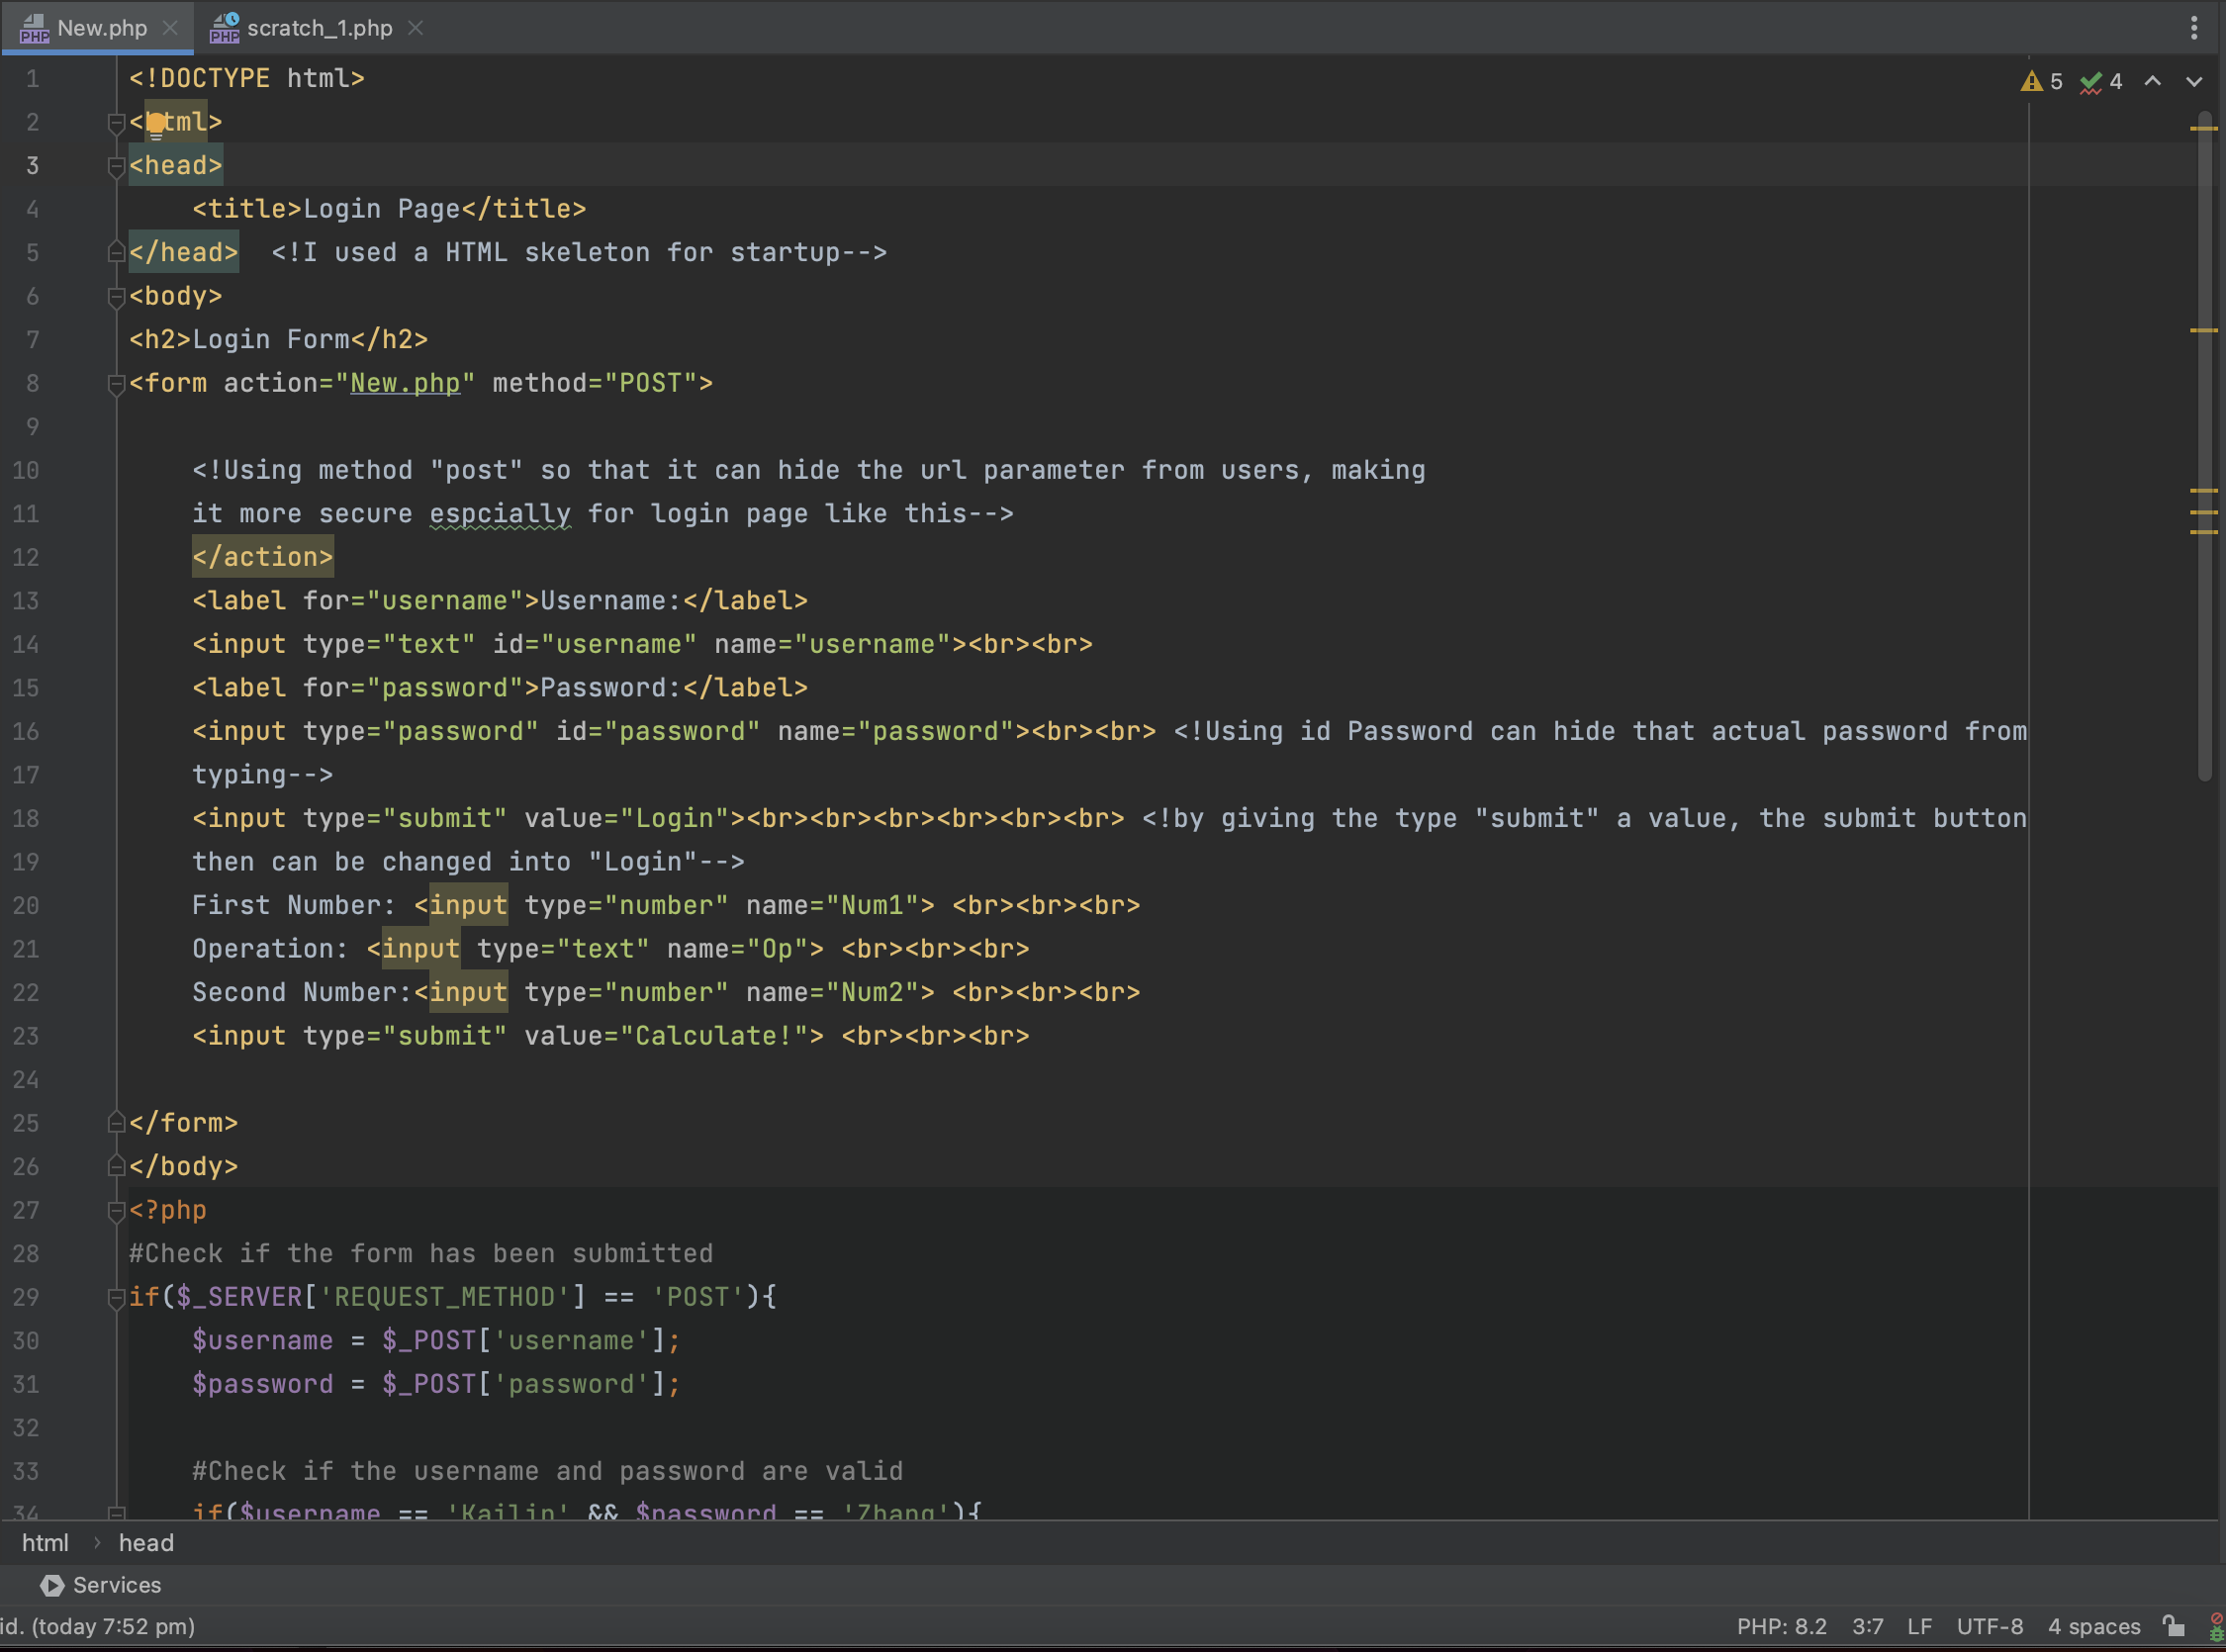
\includegraphics[width=1\textwidth]{1}
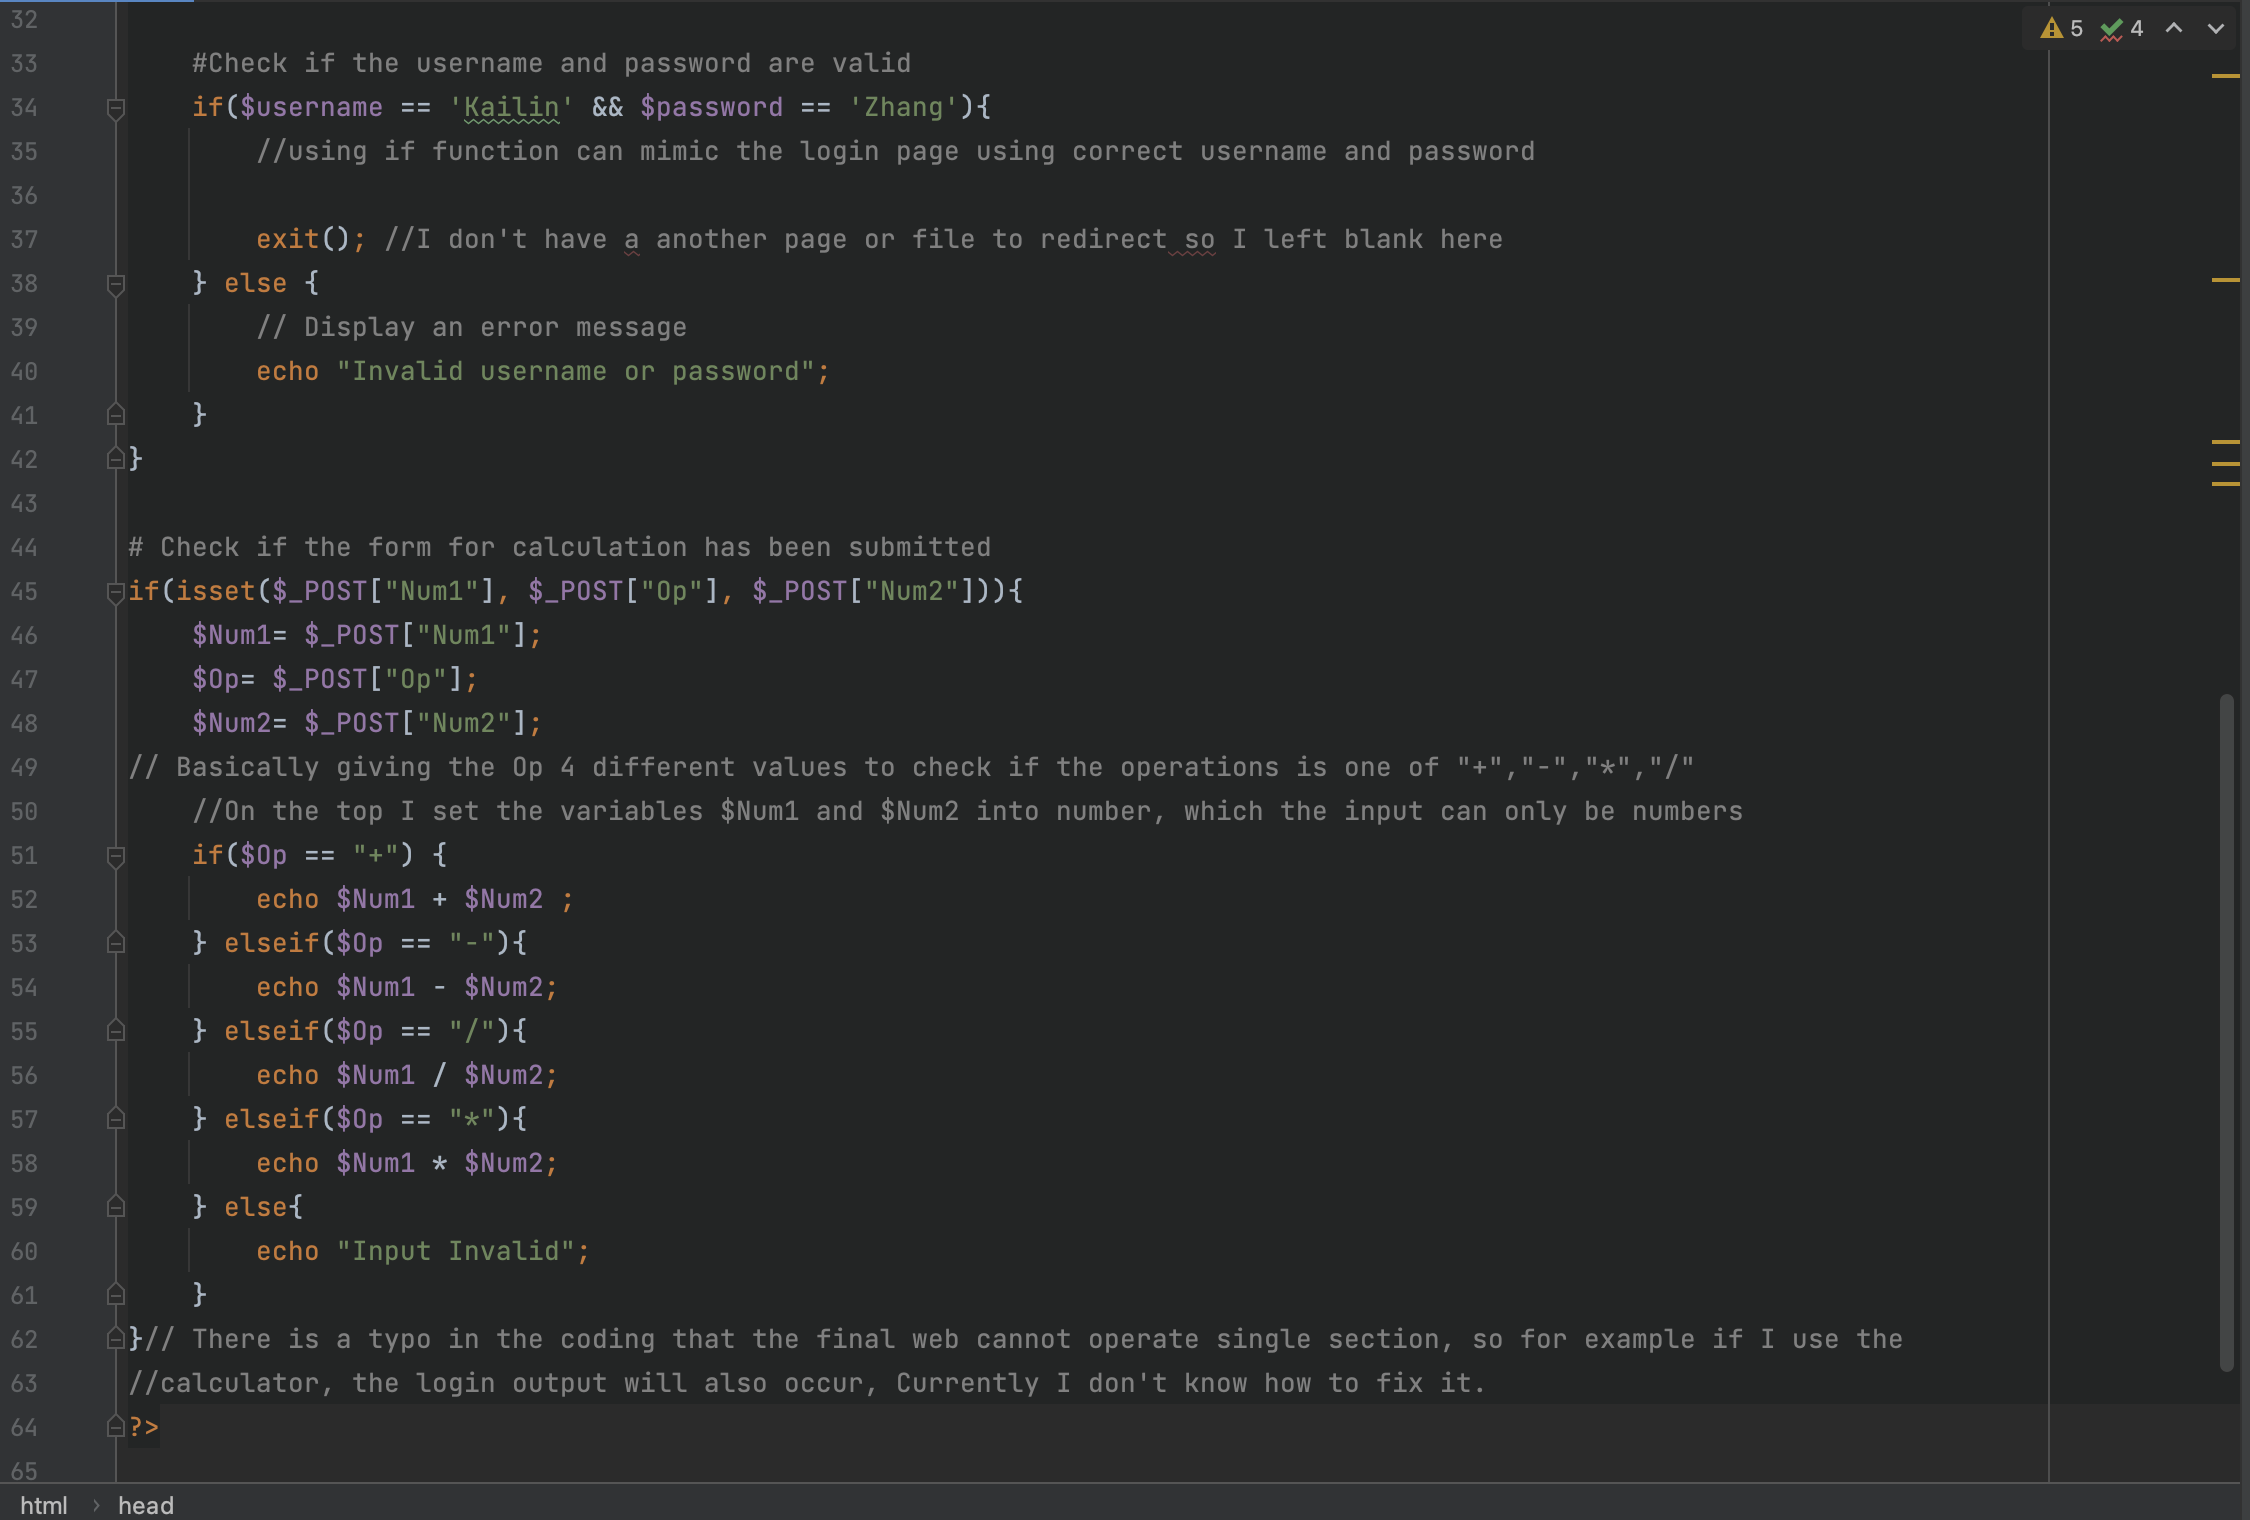
\includegraphics[width=1\textwidth]{2}

%=============================================================================
\newpage
\section{Level B: Basic Application}
\subsection{Level B Demonstration}
So my topic that I chose was PHP, so for level b I developed some what knowledge in XAMPP which is a web sever that supports PHP language and also MySQL database. I used XAMPP in level b to generate a local sever for me to use php html css with the MySQL database to create a sign up web page that can store the users' input(usernames and password)
Meanwhile, I have also used Phpadmin to store the login data using MySQL.
\subsection{Application artifacts}

I have created a simple website with a sign-up page that can store user input in a database. The process I followed is as follows:

\begin{enumerate}
    \item Downloaded XAMPP, a cross-platform server, to create a local host on my laptop.
    \item Launched Apache and MySQL inside XAMPP to create a local server that supports PHP and MySQL databases.
    \item Downloaded phpMyAdmin and inserted it into the XAMPP "htdocs" folder to help manage the MySQL database.
    \item Created a MySQL database and user with all privileges using phpMyAdmin.
    \item Created a table under the database structure to store users' input usernames and passwords.
    \item Used Visual Studio Code to create PHP files for connecting to the database and processing the sign-up form.
    \item Incorporated an HTML sign-up form template from the getbootstrap website, and used the "post" method for secure data transmission.
    \item Utilized prepared statements with \texttt{mysqli\_prepare()} to prevent SQL injection attacks.
    \item Implemented error handling for cases when user information is already stored in the database.
\end{enumerate}

The resulting website has a simple structure with a sign-up page that stores user input in the database. If the user's information is already stored in the database, it will detect and output an error; otherwise, it will store the information successfully.

Here is a code snippet from the PHP file for connecting to the MySQL database:

\begin{lstlisting}[language=php]
<?php
// Connection details
$hostname = "SQL;
$username = "k";
$password = "123";
$database = "registration";

// Create connection
$connection = mysqli_connect($hostname, $username, $password, $database);

// Check connection
if (!$connection) {
    die("Connection failed: " . mysqli_connect_error());
}
?>
\end{lstlisting}

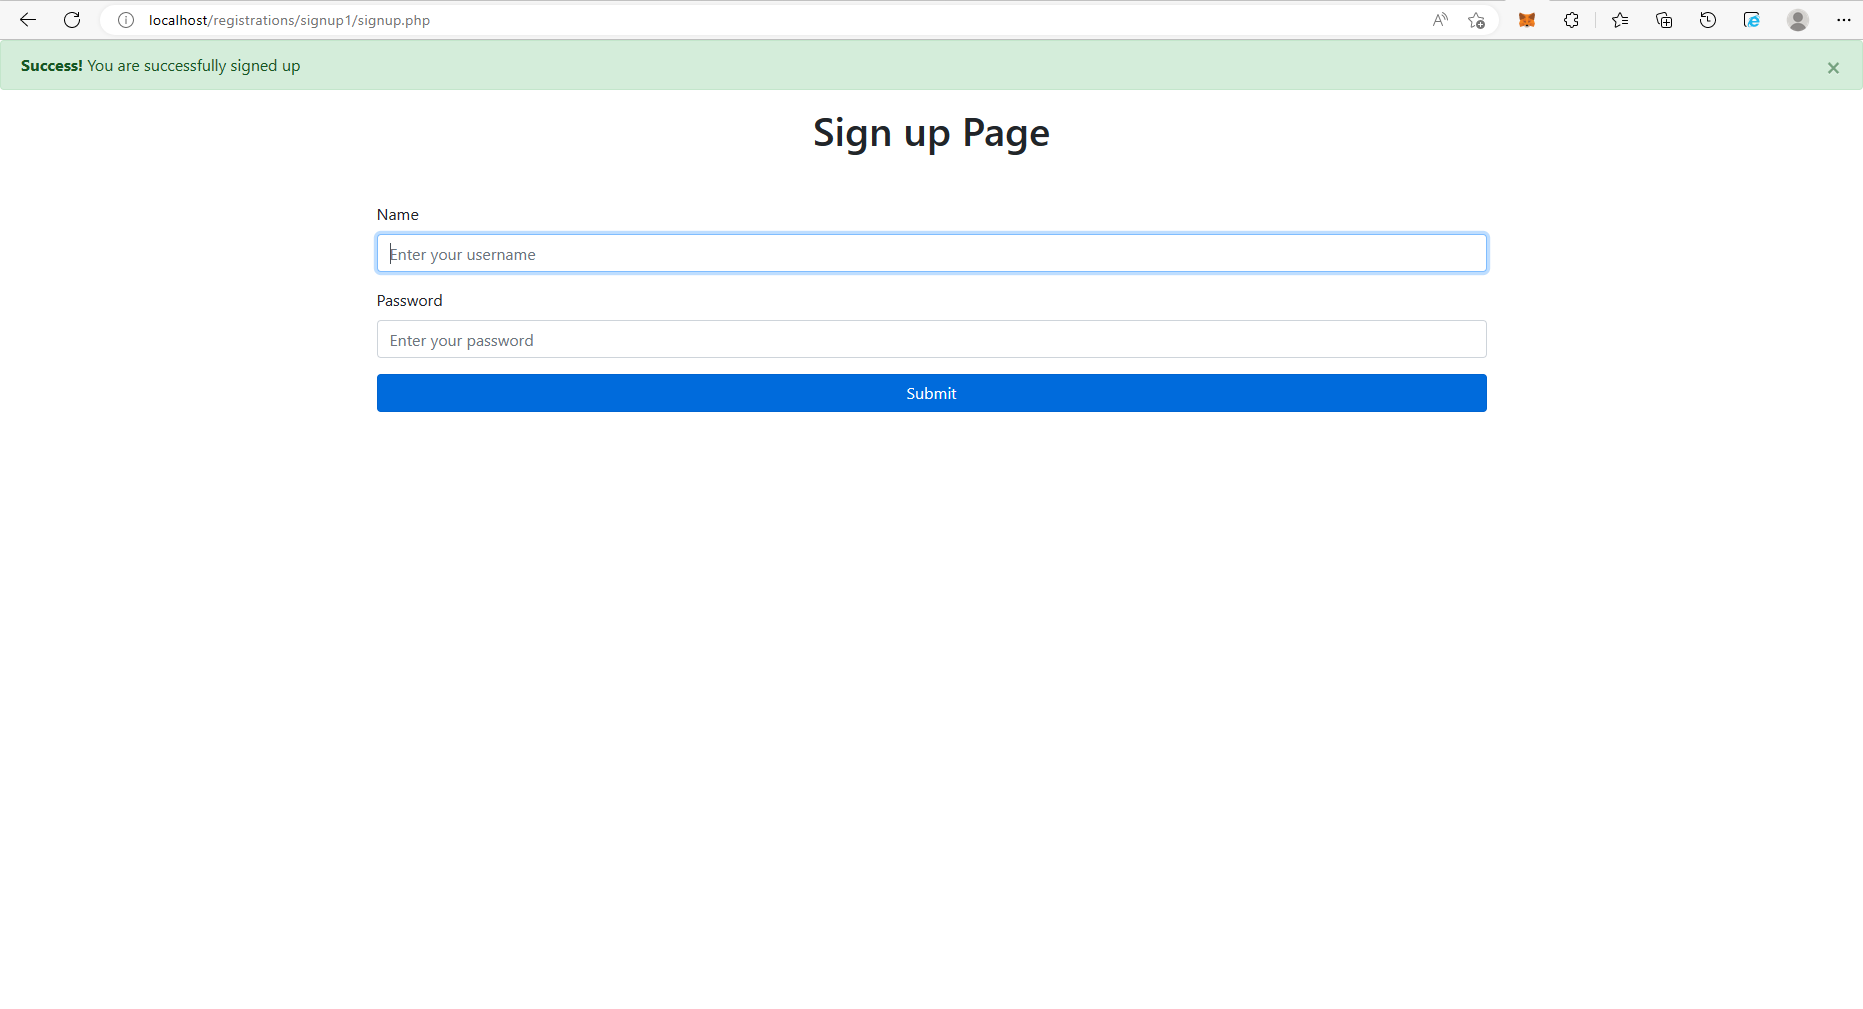
\includegraphics[width=0.5\textwidth]{Local}
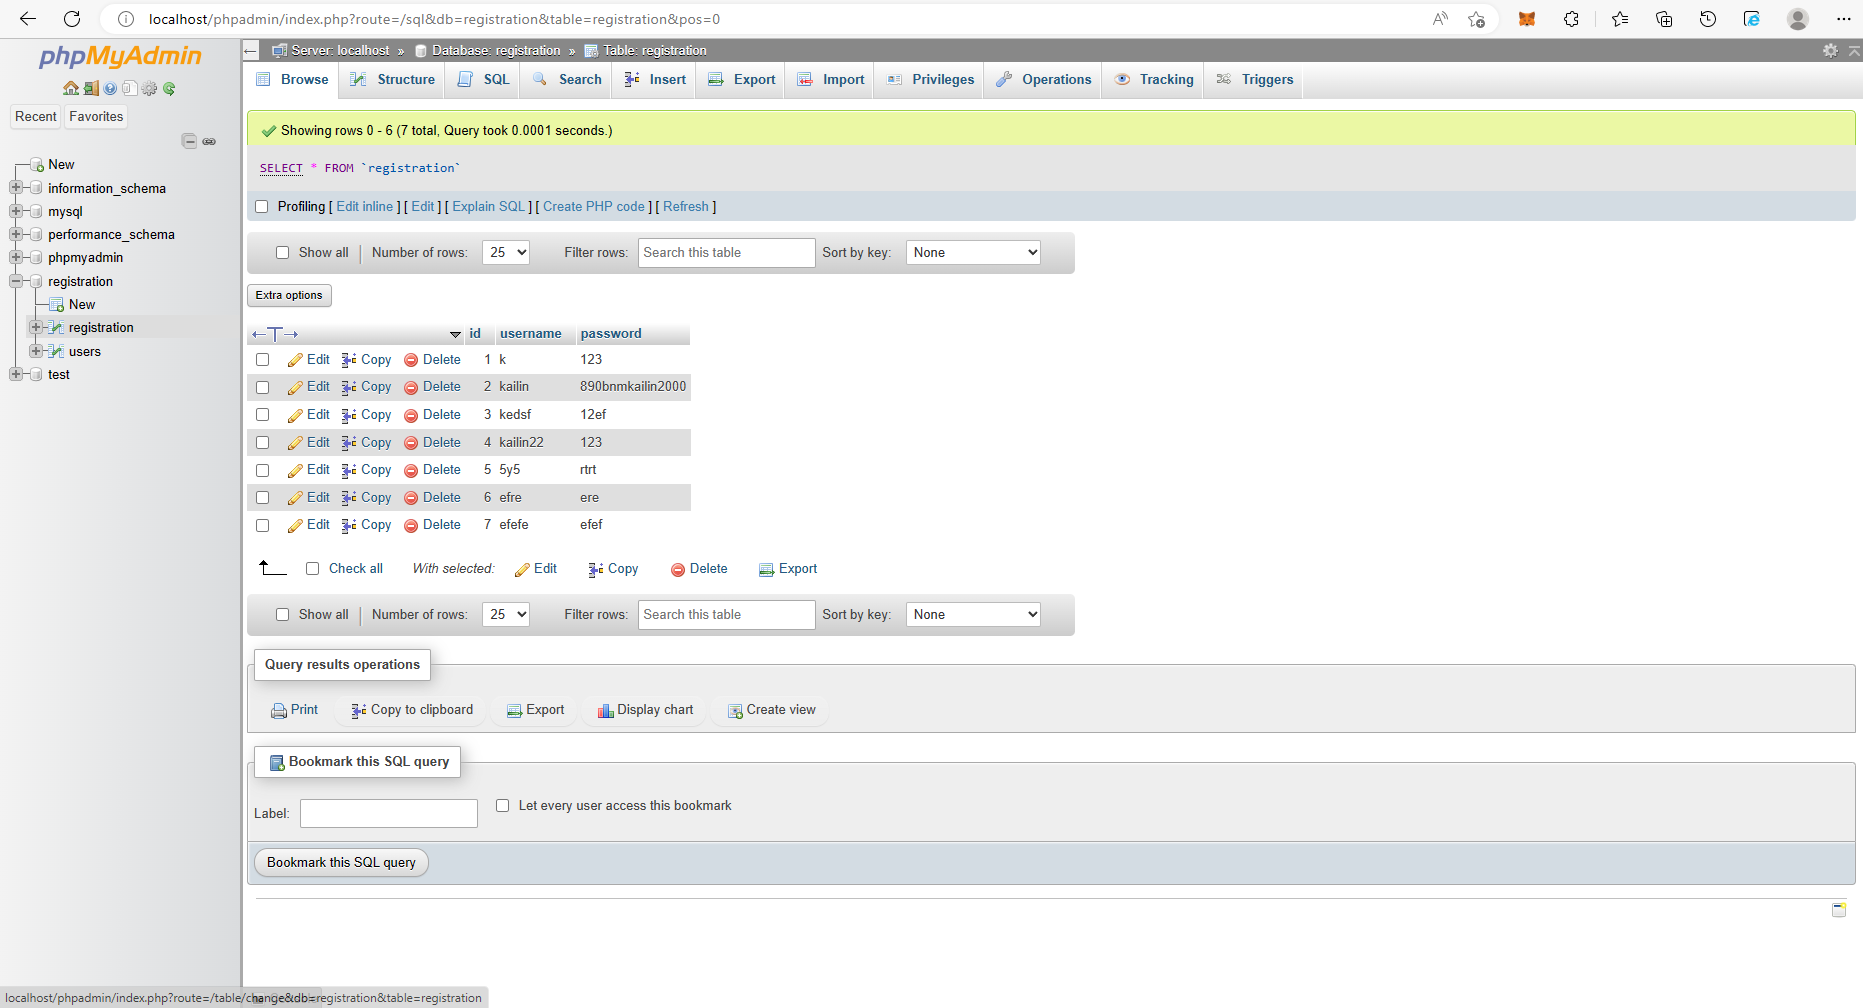
\includegraphics[width=0.5\textwidth]{PHPadmin}
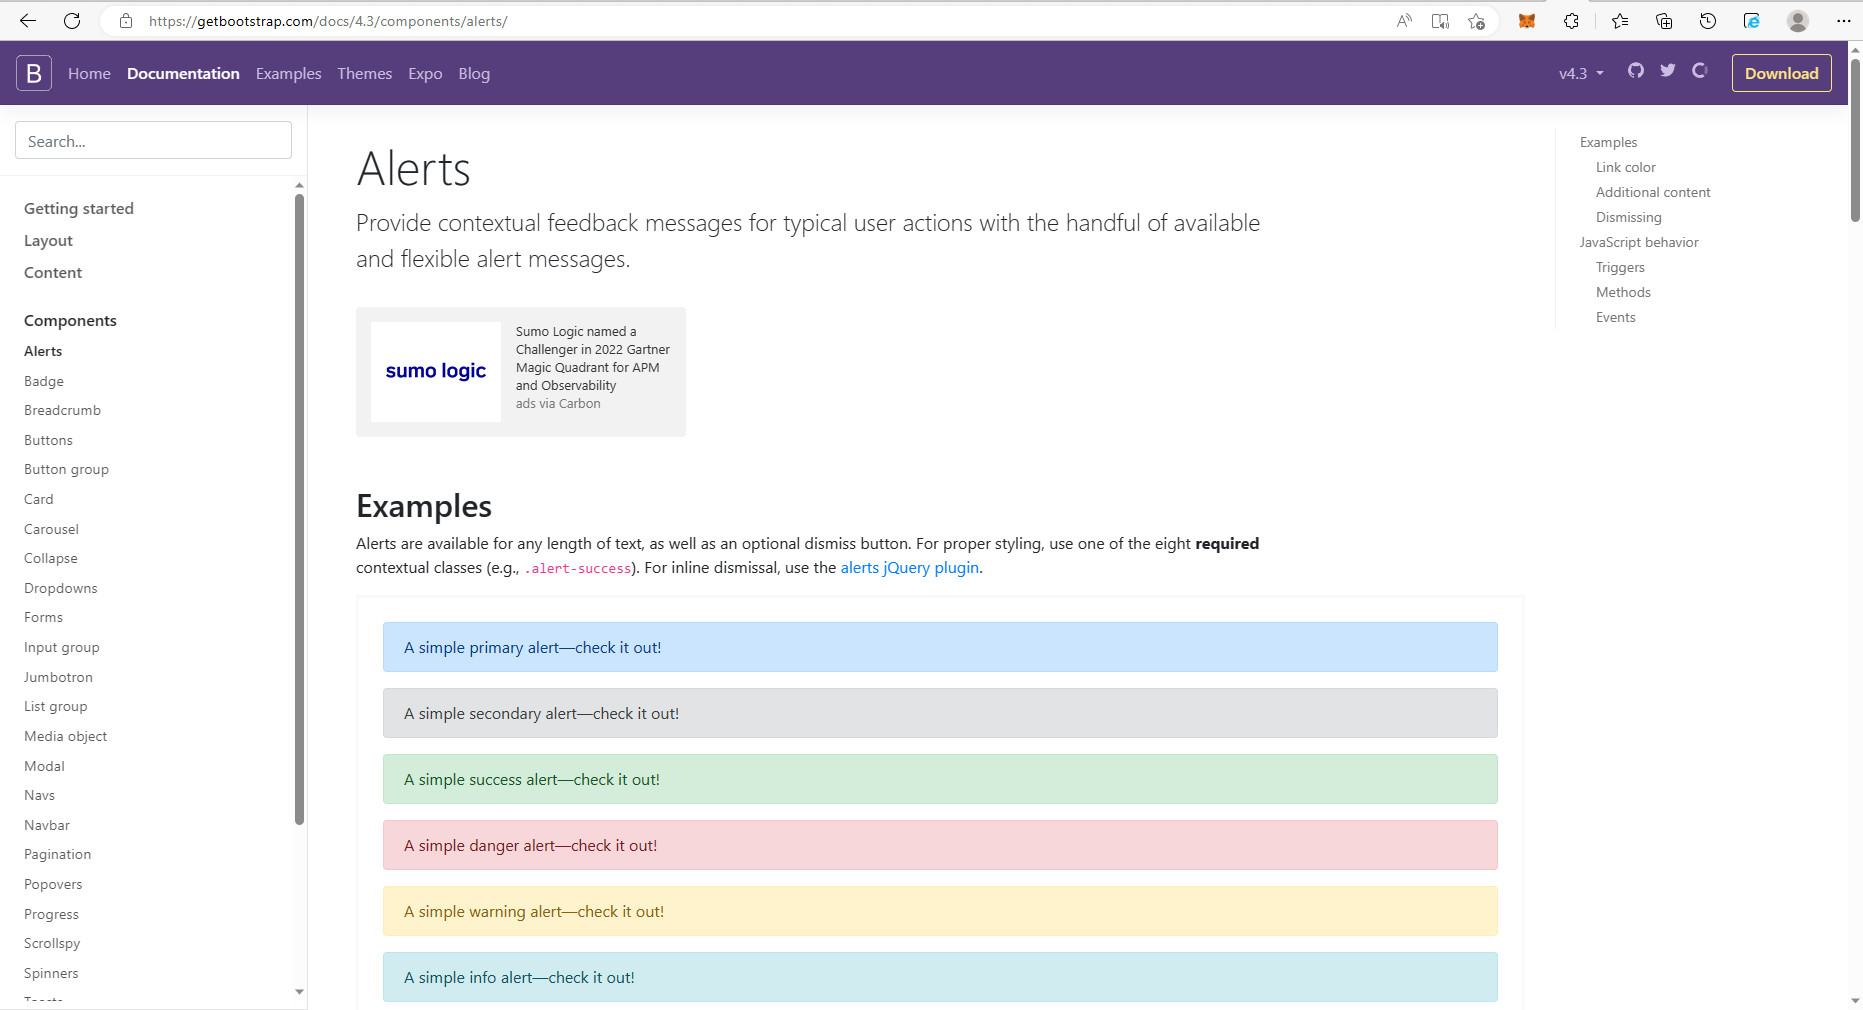
\includegraphics[width=0.5\textwidth]{getbootstrap}
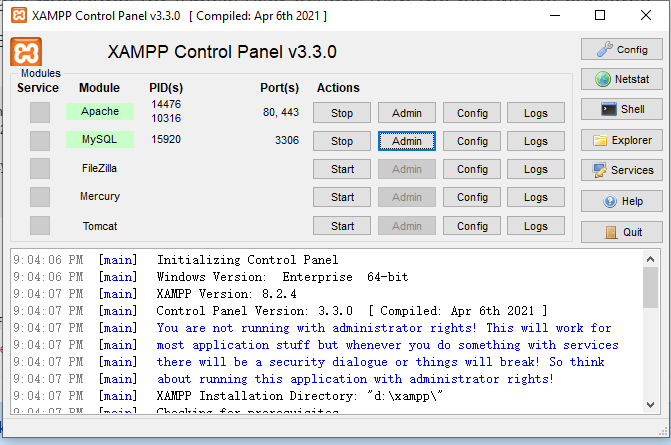
\includegraphics[width=0.5\textwidth]{XAMPP}

%=============================================================================


\newpage
\section{Level C: Deeper Understanding}

\subsection{Strengths}
PHP, a server-side scripting language, is favored for its simplicity, flexibility, and strong community support. Its syntax is straightforward, promoting quick learning and real-world application even for novices. PHP excels in text processing - a critical aspect in web development - and is backed by an extensive range of libraries, extensions, and frameworks, contributed by its vibrant global community. These factors, combined with immediate community support for technical issues, make PHP a versatile and accessible tool for diverse programming tasks\cite{Ryadel}.


\subsection{Weaknesses}
While PHP remains a robust language for web development, it faces a decline in popularity, with newer developers gravitating towards languages like Python for its simplicity and modern capabilities. This trend may result in higher costs for PHP-based products as the number of novice developers decreases. Despite having numerous libraries, PHP lacks specific ones dedicated to emerging trends like AI, limiting its competitiveness against languages like Python. Furthermore, security has been a longstanding concern for PHP, with vulnerabilities potentially being exploited by malicious entities before fixes are implemented\cite{Journal}.

\subsection{Usefulness}
Usefulness A scenario where PHP shines is the development of a dynamic e-commerce website. For instance, an online clothing store needs a site that can handle customer registration, product display, shopping cart functionality, and payment processing. PHP, being server-side, excels at handling such data-driven tasks. Additionally, its integration with database systems like MySQL enables efficient storage and retrieval of product details and customer information. Moreover, with PHP's text processing strengths, it becomes easier to create SEO-friendly URLs and content, enhancing the store's visibility on search engines.

\subsection{Key Question 1}
Processing data server-side with PHP has a few advantages over client-side JavaScript processing. First, PHP can interact directly with the server's file system and databases, which isn't possible in JavaScript due to browser security restrictions. Second, as PHP code is run server-side, it's hidden from the end user, enhancing security for sensitive operations such as password checks. Lastly, server-side processing with PHP ensures that the functionality of your website doesn't depend on the client's browser capabilities or settings. Thus, it provides a more consistent and controlled environment for running your code\cite{Vs}.

\subsection{Key Question 2}
Despite PHP's versatility, it may not be the best choice for certain types of applications. Highly computationally intensive applications, like those involved in scientific computing or big data analysis, might be better served by languages like Python or Java, which have extensive libraries and frameworks tailored to these tasks. Moreover, for real-time applications like instant messaging or gaming, Node.js might be a more suitable choice due to its non-blocking, event-driven architecture. Lastly, while PHP can be used for mobile app backend, it's not used for writing the app itself, where languages like Swift (for iOS) or Kotlin (for Android) are more applicable.


%=============================================================================

\newpage
\section{Level D: Evolution of skills}
\vspace{5mm}
\subsection{Level D Demonstration}
So I basically made a website using html to make the border and created a separate style sheet made with CSS. The image inserted into the html file is from a local database with the help of Mysql, I also connected to a local sever with the help of XAMPP. Finally inside the html I used the php scripting language to finalise the final web page.

\subsection{Application artifacts}
	So basically I first downloaded the XAMPP, which is application that supports for you to create a local sever that will able to process an HTTP request and deliver HTML pages to my web browser. It also can support for MySQL, which is a database management system. Then I downloaded PHPmyadmin to help me manage the database. to insert, edit, and delete data. I created a file folder for this project, one is the indext.php: which is a simple html skeleton embedded with php scripting language to code the outer layer of the website. For html part, I used bootstrap for the basic border. Then I used php to include my "Header", "Footer" and "connect" file. I have also made a separate css file named style, it is for the font style, image size and other style related for the website. For the image that I used in the web, I have stored in the Myphpadmin which have linked in my index for use in php language.

\subsection{Alternative tools/technologies}

	Node.js is mainly aimed for server-side scripting language.It allows Javascript run on server instead of web page, enabling full -stack JavaScript.development. It can also generate dynamic page content, which is faster due to it eliminates the waiting, and simply continues with the next request. Node.js can also cope with MongoDB, which is aNoSQL database in order to edit, store data and use it on its server\cite{W32}.
	Django is a versatile web framework that leverages the simplicity of Python, offering a suite of pre-built tools, thus making it a prime choice for quick web development. The beauty of Django is its adaptability; it has been utilized to construct a wide variety of websites, from social networking platforms and news sites to content management systems and wikis. When coupled with a robust database like PostgreSQL, Django effortlessly manages intricate data relations, reinforcing its practicality for diverse web development needs\cite{Django}.
\subsection{Comparative Analysis}

Describe situations in which both your topic and each of the identified alternatives would be preferred over the others (100-200 words).
PHP: PHP really stands out when the focus is on creating simple, server-side websites quickly. It shines in environments where the host platform offers superior support for PHP compared to other technologies. It's particularly useful when the project requires integration with systems already using PHP, and it's beneficial if the team's skill set aligns strongly with PHP. Plus, the abundance of PHP-based frameworks, such as Laravel and Symfony, make it a go-to choice for projects requiring custom solutions with fewer resources.

Node.js (JavaScript): Node.js is a perfect fit for applications that need real-time responses, such as chat applications, live feeds, or collaborative tools. Its non-blocking I/O model excels at handling concurrent requests, making it extremely efficient for scenarios where multiple users interact with the server simultaneously. If the development team is proficient in JavaScript, choosing Node.js means they can use the same language for both frontend and backend, improving productivity.

Python (Django): When a project leans heavily on complex data relationships, or when readability and maintainability of code are key factors, Python and Django step up. Django’s clean, high-level abstraction of common web project tasks like URL routing, database manipulation, and template rendering means faster development cycles. Moreover, in fields like data analysis, scientific computing, and machine learning, the extensive libraries Python offers make it the preferred choice.


%=============================================================================

\newpage
\bibliographystyle{IEEEtran}
\bibliography{123}


\end{document}


\end{document}
\end{report}
